\documentclass[tikz,border=5pt]{standalone}
\usepackage[T1]{fontenc}
\usepackage{pgfplots}
\usepgfplotslibrary{groupplots}
\pgfplotsset{compat=1.18}
\definecolor{allowblue}{RGB}{0,88,138}
\definecolor{denyred}{RGB}{163,41,47}
\definecolor{certorange}{RGB}{166,95,0}
\begin{document}
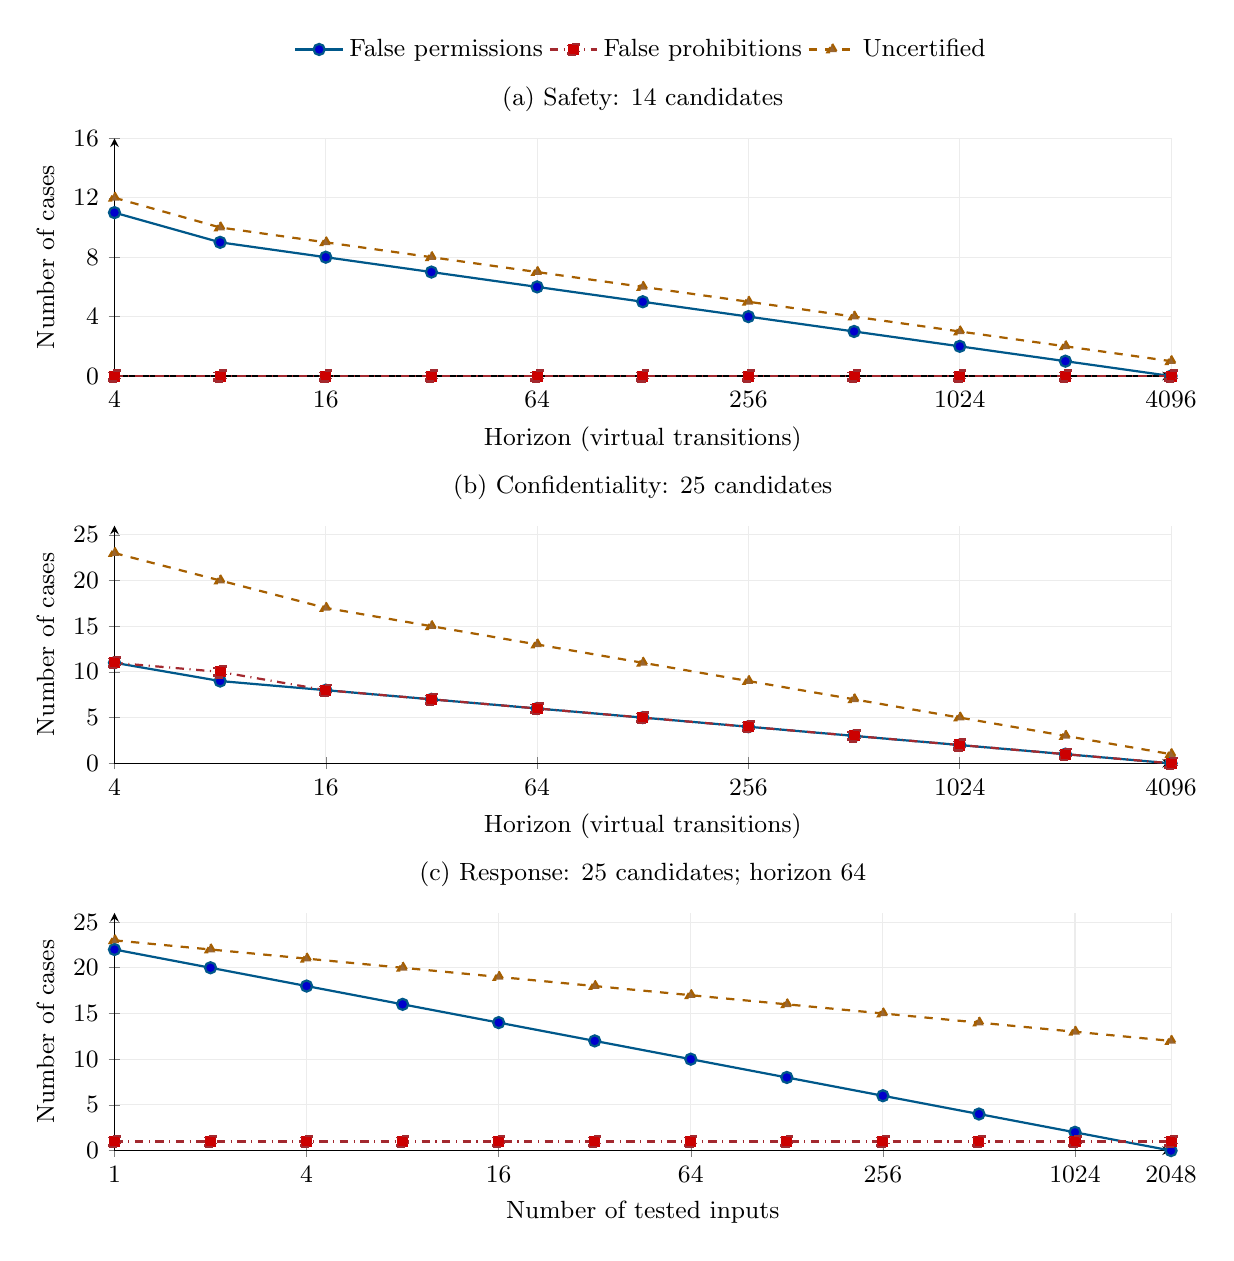
\begin{tikzpicture}
\begin{groupplot}[
 group style={group size=1 by 3,vertical sep=1.9cm},
 width=15cm,height=4.6cm,xmode=log,log basis x=2,
 axis lines=left,ymin=0,grid=major,grid style={gray!15},
 ylabel={Number of cases},title style={font=\small},
 tick label style={font=\small},label style={font=\small},
 legend style={at={(0.5,1.28)},anchor=south,legend columns=3,draw=none,font=\small}]
\nextgroupplot[title={(a) Safety: 14 candidates},ymax=16,ytick={0,4,8,12,16},
 xmin=4,xmax=4096,xtick={4,16,64,256,1024,4096},
 xticklabels={4,16,64,256,1024,4096},xlabel={Horizon (virtual transitions)}]
\addplot+[color=allowblue,mark=*,solid,thick,mark size=2pt] coordinates {(4,11) (8,9) (16,8) (32,7) (64,6) (128,5) (256,4) (512,3) (1024,2) (2048,1) (4096,0)};
\addlegendentry{False permissions}
\addplot+[color=denyred,mark=square*,dashdotted,thick,mark size=2pt] coordinates {(4,0) (8,0) (16,0) (32,0) (64,0) (128,0) (256,0) (512,0) (1024,0) (2048,0) (4096,0)};
\addlegendentry{False prohibitions}
\addplot+[color=certorange,mark=triangle*,dashed,thick,mark size=2pt] coordinates {(4,12) (8,10) (16,9) (32,8) (64,7) (128,6) (256,5) (512,4) (1024,3) (2048,2) (4096,1)};
\addlegendentry{Uncertified}
\nextgroupplot[
 title={(b) Confidentiality: 25 candidates},ymax=26,ytick={0,5,10,15,20,25},
 xmin=4,xmax=4096,xtick={4,16,64,256,1024,4096},
 xticklabels={4,16,64,256,1024,4096},xlabel={Horizon (virtual transitions)}]
\addplot+[color=allowblue,mark=*,solid,thick,mark size=2pt] coordinates {(4,11) (8,9) (16,8) (32,7) (64,6) (128,5) (256,4) (512,3) (1024,2) (2048,1) (4096,0)};
\addplot+[color=denyred,mark=square*,dashdotted,thick,mark size=2pt] coordinates {(4,11) (8,10) (16,8) (32,7) (64,6) (128,5) (256,4) (512,3) (1024,2) (2048,1) (4096,0)};
\addplot+[color=certorange,mark=triangle*,dashed,thick,mark size=2pt] coordinates {(4,23) (8,20) (16,17) (32,15) (64,13) (128,11) (256,9) (512,7) (1024,5) (2048,3) (4096,1)};
\nextgroupplot[
 title={(c) Response: 25 candidates; horizon 64},ymax=26,ytick={0,5,10,15,20,25},
 xmin=1,xmax=2048,xtick={1,4,16,64,256,1024,2048},
 xticklabels={1,4,16,64,256,1024,2048},xlabel={Number of tested inputs}]
\addplot+[color=allowblue,mark=*,solid,thick,mark size=2pt] coordinates {(1,22) (2,20) (4,18) (8,16) (16,14) (32,12) (64,10) (128,8) (256,6) (512,4) (1024,2) (2048,0)};
\addplot+[color=denyred,mark=square*,dashdotted,thick,mark size=2pt] coordinates {(1,1) (2,1) (4,1) (8,1) (16,1) (32,1) (64,1) (128,1) (256,1) (512,1) (1024,1) (2048,1)};
\addplot+[color=certorange,mark=triangle*,dashed,thick,mark size=2pt] coordinates {(1,23) (2,22) (4,21) (8,20) (16,19) (32,18) (64,17) (128,16) (256,15) (512,14) (1024,13) (2048,12)};
\end{groupplot}
\end{tikzpicture}
\end{document}
